\documentclass[unicode,pdfcover]{scutthesis}

\usepackage[unicode=false,bookmarks=true,bookmarksnumbered=true,bookmarksopen=false,
 breaklinks=false,pdfborder={0 0 1},backref=false,colorlinks=true]
 {hyperref}

%%%%以下包可根据需要插入,基本涵盖所需内容。
\usepackage{multirow}%画表格推荐先在Excel简单制表,然后复制到该网页{Create LaTeX tables online https://tablesgenerator.com/}自动生成tex代码再粘贴过来(按需进一步简单修改)。
%\usepackage{arydshln}
%\usepackage{amsmath}%公式推荐使用WinEdt 10.3自带的IDE插入,公式外的特殊字符请使用$$括起来。
%\usepackage[算法]{algorithm}%算法二字可中文显示“算法”
%\usepackage{algorithmic}
\usepackage{lscape}%横放图表时用到
%\usepackage{longtable}%跨页表格用到

\hypersetup{pdftitle={学位论文标题},
 pdfauthor={你的名字},
 pdfsubject={华南理工大学博士学位论文},%博士请使用该设置,此为偶数页页眉字样
 %pdfsubject={华南理工大学硕士学位论文},%硕士请使用该设置,此为奇数页页眉字样
 pdfkeywords={关键字1, 关键字2},
 linkcolor=blue, anchorcolor=black, citecolor=black, filecolor=magenta, menucolor=red, urlcolor=blue}

\begin{document}
\maketitle

\frontmatter

\begin{abstractCN}
本文用于测试scutthese.cls的使用,主要包括xelatex是否正常可调用,中文字体是否显示之前,pdf标签是否正确显示。大部分Windows系统缺乏“楷体\_GB2312.ttf”字体注册,请先安装该字体。封面请按要求修改Word文档 thesis\_cover.doc 中相应内容,并另存为pdf格式。

本文档基于《华南理工大学学位论文Latex/Lyx模板》\cite{2016Scutthesis}(来自https://github.com/alwintsui/scutthesis),增删内容如下:
\begin{itemize}
  \item 补充了部分图、表和公式的演示例子。
  \item 修改了scutthesis.bst,使得即便reference.bib里面有多余未引用条目,在Windows 的Texlive(2018)下依然能够顺利编译通过。
  \item 修改了结论在chapterx命令下,偶数页显示上一章标题的错误。
  \item 修改了附录中图、表和公式接着正文章节序号编号的错误。
  \item 修改了在Windows下致谢最后名称和日期没有右对齐的格式。
\end{itemize}


\end{abstractCN}
\keywordsCN{\LaTeX{};排版;论文}

\begin{abstractEN}
This article tests the usage of scutthese.cls \LaTeX{} typesetting.
\end{abstractEN}
\keywordsEN{\LaTeX{};  Typesetting; Paper}


\tableofcontents{}%自动生成章节内容目录,要第二次编译才能生成

%\listoftables%自动生成表格目录,要第二次编译才能生成。如需使用,请去掉前面注释%。若标题含有文献引用,请先注释进行BibTex编译生成bbl文件后,再使用该命令。

%\listoffigures%自动生成图目录,要第二次编译才能生成。如需使用,请去掉前面注释%。若标题含有文献引用,请先注释进行BibTex编译生成bbl文件后,再使用该命令。

\mainmatter

\chapter{绪论}
Tex排版\cite{knuth1986thetexbook}是由Knuth最早发明,后来人们对其扩展了大量宏包以增强其功能,而且设计了多种不同的Tex专业引擎,其中内置了许多常用的Tex宏包,如\LaTeX{}\cite{goossens1994thelatex};内核不同的新TEX引擎,如XeTex(包含LaTex宏包的称为XeLaTex),它支持支持UTF-8文档编码而以pdf格式输出。

XeTex引擎使用xeCJK宏包支持中文排版,大大方便了中日韩语言用户排名。我们自定义了scutthesis.cls模板库,它是基于latex/base/book.cls进行文章结构布局,并调用了xelatex/xecjk/xeCJK.sty宏包,以UTF-8方式支持中文显示。scutthesis.cls模板库是一套“华南理工大学博士学位论文”模板。

\section{English}
Test English section name.

\section{中文}
测试中文section的标题名,中文文献引用\cite{cnproceed, wang_model_2009}。先用XeLatex编译一次,然后再用BibTex编译一次生成.bbl文件后(BibTex编译出错也没关系),Build Tree刷新一下目录、结构、引用和标签,再用XeLatex编译两次就能正常显示引用文献了。

\chapter{图表公式演示}
\section{插图演示}
多图插图演示。常见的subfigure命令改为subfloat命令。在当前.cls文件中,textwidth长度等于columnwidth的长度。图可设固定高度或固定宽度。图片名称不需要带后缀,且不应有空格。建议所有图片放到figure文件夹下面,并且命名时加上章节序号,方便管理。
\begin{figure}[htp]%括号内请标注当前图的位置设置,一般设为htp(表示here,top,page)。若没有设,编译时可能会有warnning提示,但仍能编译成功
  \centering%居中图
  \subfloat[小图1] {\label{FIG1-1}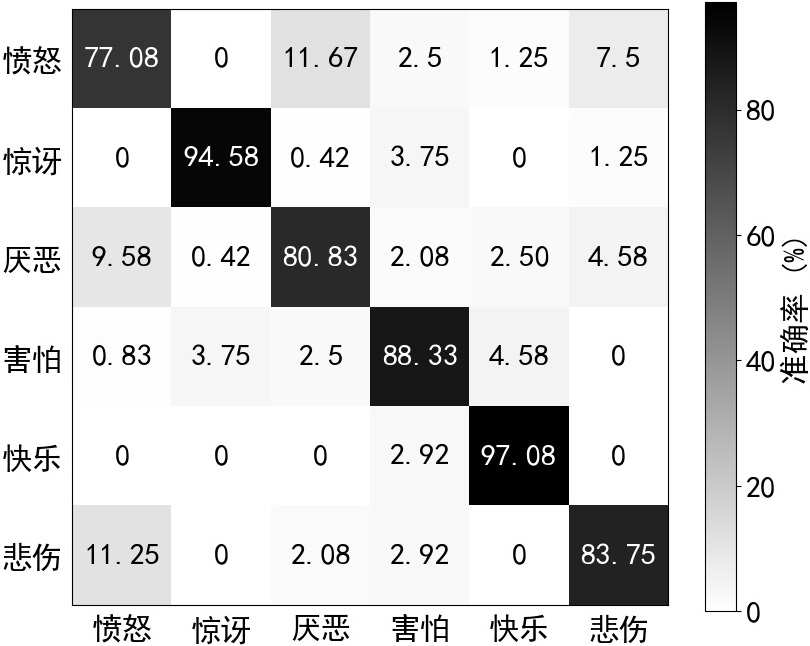
\includegraphics[height=0.2\textwidth,keepaspectratio]{figure/FIG2-1}}
  \hspace{5mm}%同排的两图间隔
  \subfloat[小图2]{\label{FIG1-2}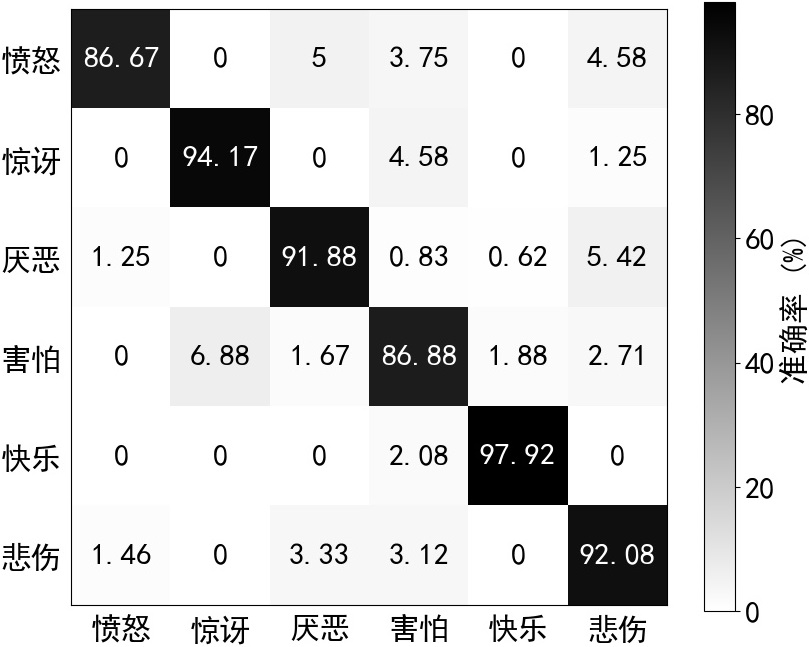
\includegraphics[height=5.5cm,keepaspectratio]{figure/FIG2-2}}\\%换行
  \subfloat[小图3]{\label{FIG1-3}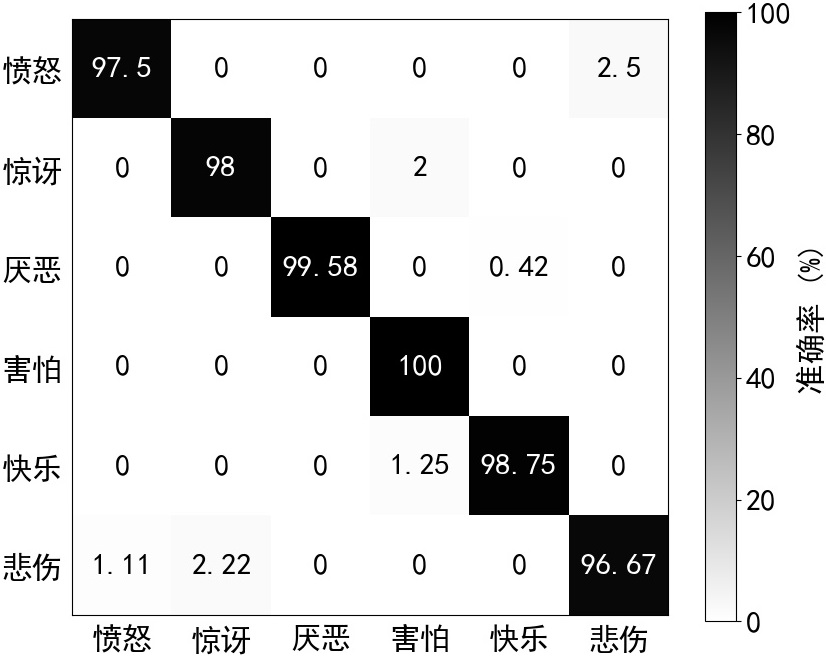
\includegraphics[width=0.3\columnwidth,keepaspectratio]{figure/FIG2-3}}
  \hspace{5mm}
  \subfloat[小图4] {\label{FIG1-4}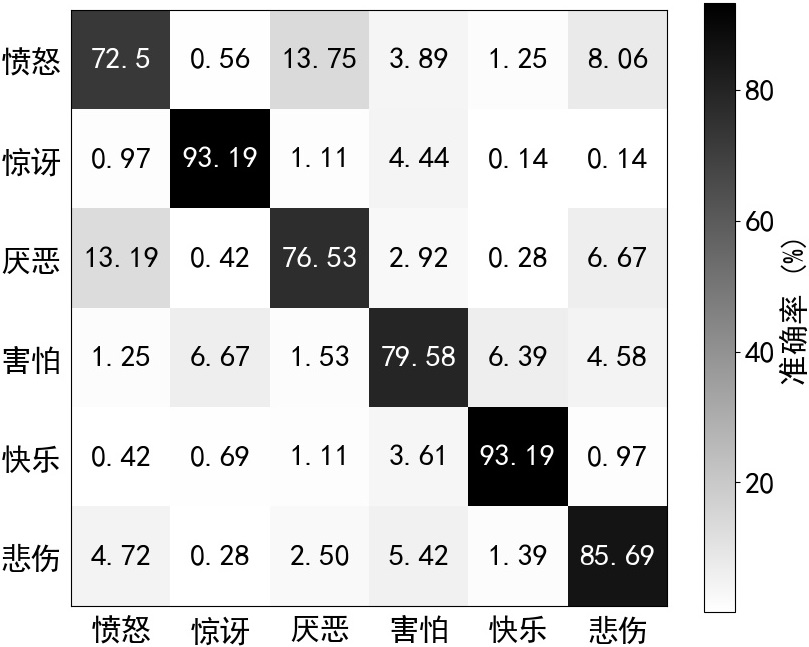
\includegraphics[width=5cm,keepaspectratio]{figure/FIG2-4}}\\
  \caption{测试多图。每个subfloat里面的label若不需引用,则可以删掉。图片目录和名称不应有空格。}
  \label{FIG-3-CM}
\end{figure}

横向插图演示。
\begin{landscape}
\begin{figure}[htp]
  \centering
  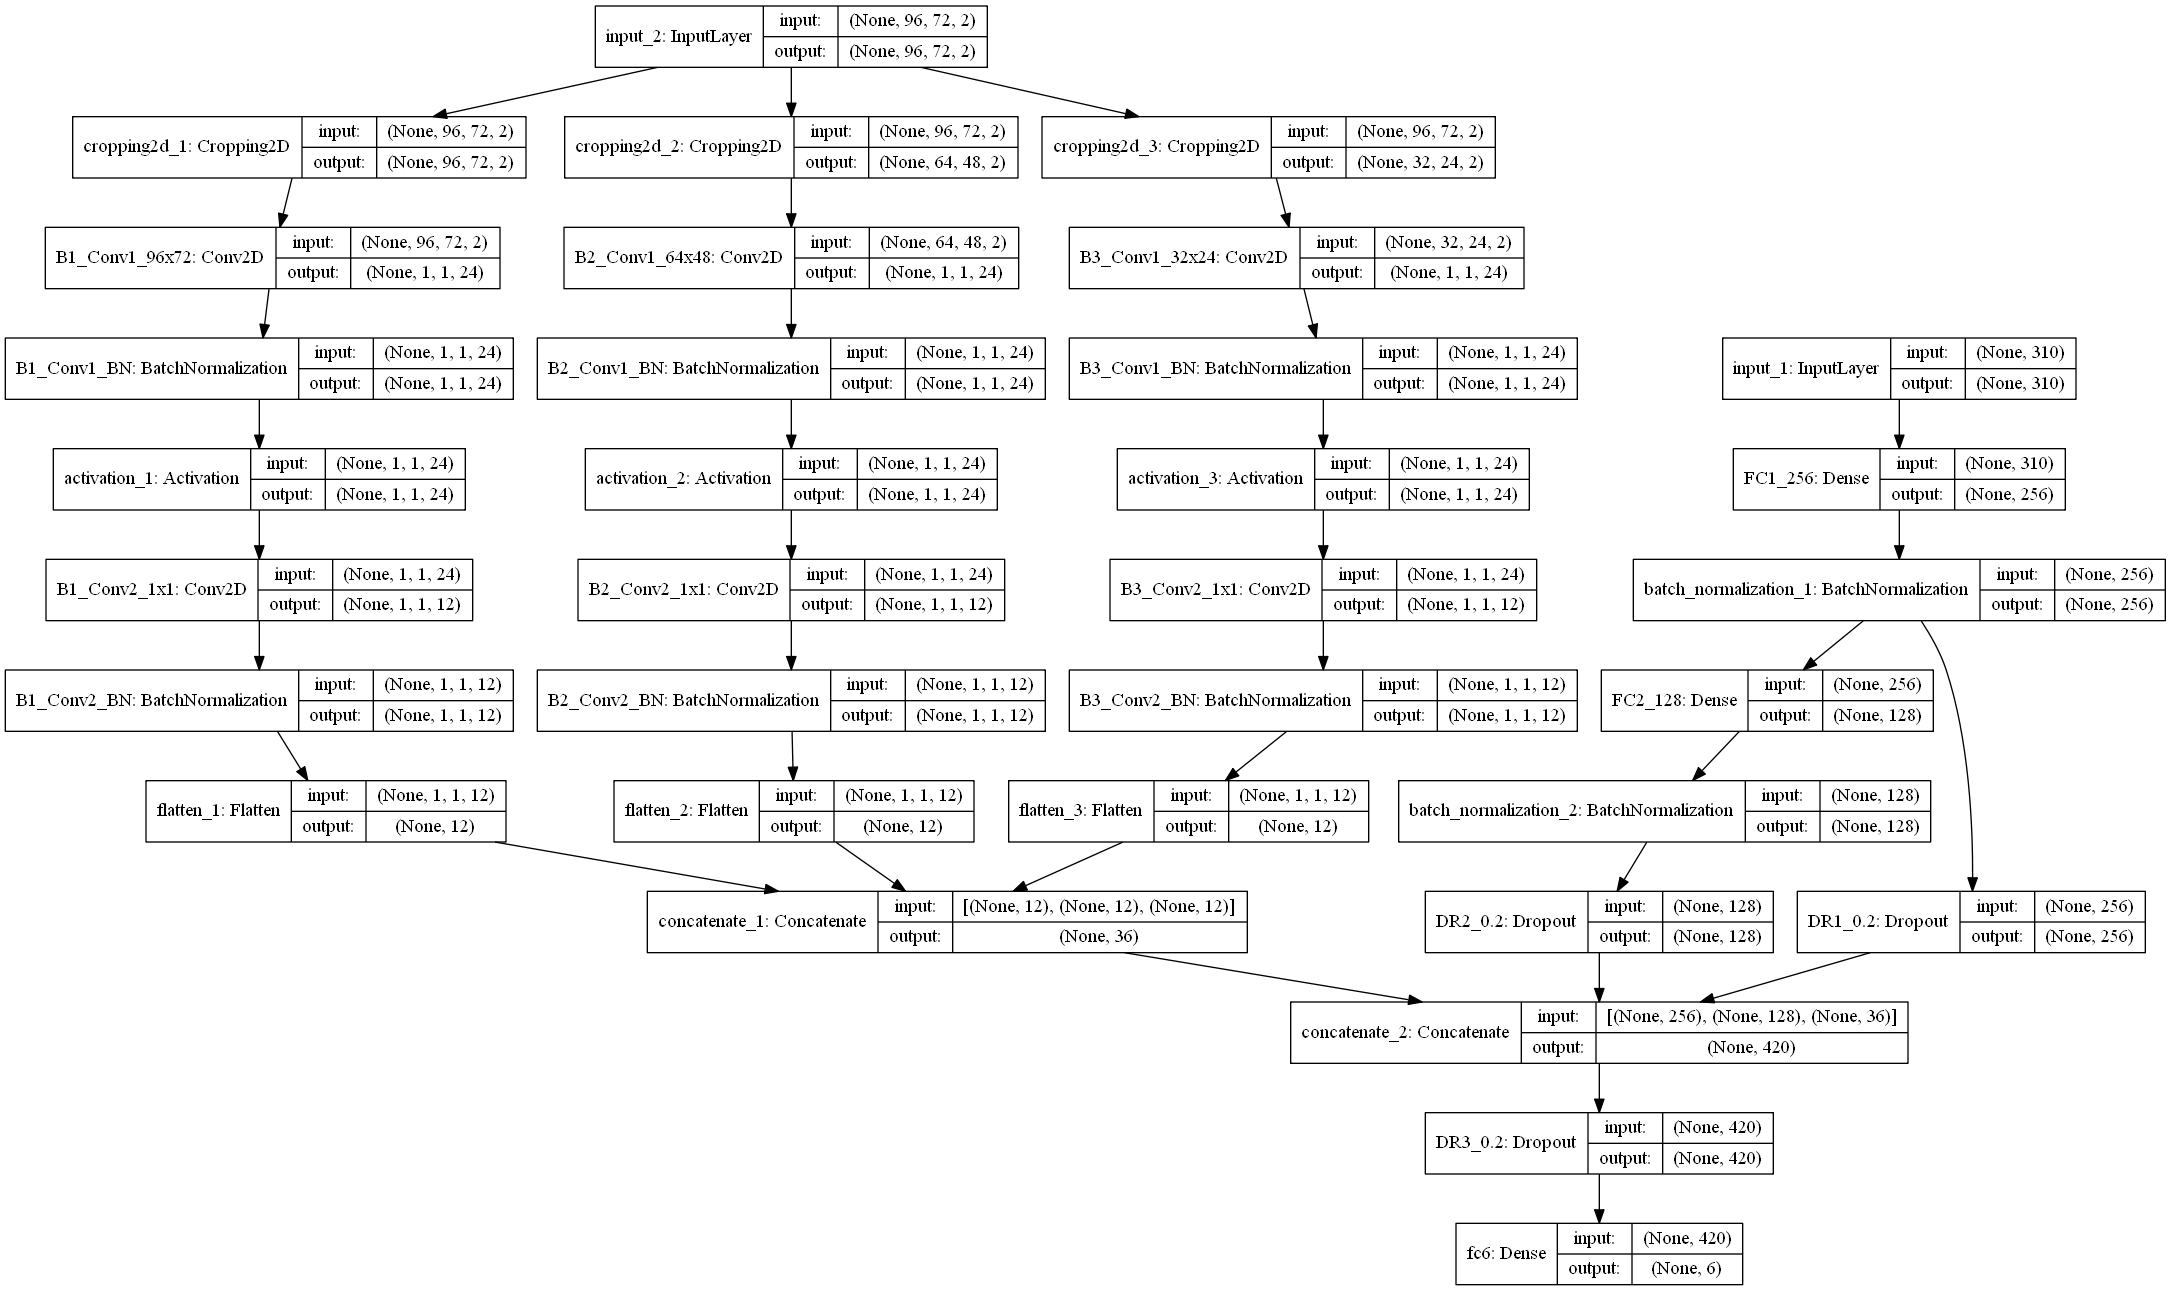
\includegraphics[width=0.8\columnwidth,keepaspectratio]{figure/FIG2-5}
  \caption{网络结构图。}
  \label{FIG-5}
\end{figure}
\end{landscape}

\section{脚注演示}
脚注示例如\footnotemark[1]所示,先作footnotemark,括号中似乎只能用整数;然后再补充footnotetext内容,建议少用,脚注太多的话注意脚注的序号。\footnotetext[1]{括号内整数要对应,编译显示的序号就为括号内的数值,并不会自动排序。}


\section{公式演示}
公式引用应在引用标签外加括号,如公式(\ref{eq1})。
\begin{equation}\label{eq1}
  a=\cos\alpha+\beta^{2}+\sqrt[n]{b_{k}+x^{y}}+\frac{c}{d}
\end{equation}

\section{表格演示}
表格不加左、右边线。表序一般按章编排,如表 \ref{T22}。\textbf{表序与表名之间应空一格},表名中不允许使用标点符号,表名后不加标点。表序与表名置于表上。
\begin{table}[htp]
\centering
\caption{表名后不加标点}
\label{T22}
\resizebox{0.75\columnwidth}{!}{%将表格缩小
\begin{tabular}{c|p{1.2cm}|p{1.2cm}|p{1.2cm}|p{1.2cm}|p{1.2cm}|p{1.2cm}|p{1.2cm}|c}\hline\hline
   \multicolumn{1}{c|}{\textbf{}} & \multicolumn{1}{c|}{\textbf{平静}} & \multicolumn{1}{c|}{\textbf{\begin{tabular}[c]{@{}c@{}}向下\\ 收缩\end{tabular}}} & \multicolumn{1}{c|}{\textbf{\begin{tabular}[c]{@{}c@{}}向中心\\ 收缩\end{tabular}}} & \multicolumn{1}{c|}{\textbf{\begin{tabular}[c]{@{}c@{}}向上下\\ 收缩\end{tabular}}} & \multicolumn{1}{c|}{\textbf{\begin{tabular}[c]{@{}c@{}}向上下\\ 拉伸\end{tabular}}} & \multicolumn{1}{c|}{\textbf{\begin{tabular}[c]{@{}c@{}}向左右\\ 拉伸\end{tabular}}} & \multicolumn{1}{c|}{\textbf{\begin{tabular}[c]{@{}c@{}}向上\\ 拉伸\end{tabular}}} & \multicolumn{1}{c}{\textbf{}} \\\hline\hline
额头 &0         &0    & 1    &-   &-          &0    &0 & \multirow{3}{*}{愤怒}    \\ \cline{2-8}
眼睛      &0 &0    & 1    &0   &-          &0    &0 &      \\ \cline{2-8}
嘴巴    & 1        &0    & 1     &0   &0          &0    &0 &      \\ \hline\hline
额头 &0 &0    & 1     &0   &0          &0    &0 & \multirow{3}{*}{厌恶}  \\ \cline{2-8}
眼睛      &0 &0    & 1     &0   &0          &0    &0 &      \\ \cline{2-8}
嘴巴    &1 &0    &0      & 1           & 0         &0    &0 &      \\ \hline\hline
\end{tabular}
}
\end{table}

画表格推荐先在Excel简单制表,然后复制到该网页{Create LaTeX tables online https://tablesgenerator.com/}自动生成tex代码再粘贴过来(按需进一步简单修改)。表格应采用小号字体,在没有缩放前提下表格内字体会偏大,所以应在表格$\setminus$begin$\{table\}$下方添加$\setminus small$命令,如表 \ref{T23}所示。
\begin{table}[htp]
\small%表格采用小号字体,若是没有缩放,则建议使用该设置
\centering
\caption{三角形集合}
\label{T23}
\begin{tabular}{c|ccccc}\hline
 集合 & \multicolumn{5}{c}{三角形点集索引值} \\ \hline
\multirow{3}{*}{$TriS_{e}$} & [17, 19, 21] & [17, 19, 27] & [27, 37, 41] & [41, 19, 27] & [41, 17, 21] \\ %\cline{2-6}
                      & [26, 24, 22] & [26, 24, 27] & [27, 44, 46] & [46, 24, 27] & [46, 26, 22] \\ %\cline{2-6}
                      & [41, 21, 27] & [17, 41, 27] & [46, 22, 27] & [26, 46, 27] &            \\ \hline
\multirow{4}{*}{$TriS_{m}$} & [4, 5, 48]   & [12, 11, 54] & [62, 66, 48] & [62, 66, 54] & [12, 11, 62] \\ %\cline{2-6}
                      & [4, 5, 66]   & [12, 11, 66] & [4, 5, 51]   & [12, 11, 51] & [4, 5, 62]   \\ %\cline{2-6}
                      & [51, 57, 48] & [51, 57, 54] & [4, 5, 57]   & [12, 11, 57] & [62, 66, 5]  \\ %\cline{2-6}
                      & [62, 66, 12] & [62, 66, 4]  & [62, 66, 11] &             &             \\ \hline
\end{tabular}
\end{table}


\chapterx{结\quad 论}
\sethead[][{\headfont{}\thesissubject}][] % 重设页眉偶数页
  {}{{\headfont{}结\quad 论}}{} % 重设页眉奇数页

我们测试了自定义的scutthesis.cls模板库的中英文显示效果。使用了XeLaTex而不是\LaTeX{}的Tex编译引擎。
正确安装XeTex(XeLaTex)后,此文正常编译后为pdf文件,其的中英文内容、标题和pdf标题都应该显示正常。


\backmatter

\bibliographystyle{scutthesis}%参考文献格式文件,scutthesis.bst
\bibliography{reference}%收录参考文献的bib文件,reference.bib,如需要换成


\appendix{附录}
%重新设置表、图、公式的序号和格式,否则接着前面的继续编号       added by YYS
\setcounter{table}{0}
\setcounter{figure}{0}
\setcounter{equation}{0}
\renewcommand{\theequation}{\textbf{A}-\arabic{equation}}%格式为A开头加序号,如A-1,A-2
\renewcommand{\thetable}{\textbf{A}-\arabic{table}}%格式为A开头加序号,如A-1,A-2
\renewcommand{\thefigure}{\textbf{A}-\arabic{figure}}%格式为A开头加序号,如A-1,A-2
%


\section{Ubuntu Linux系统下中文字体的安装}
\label{sec:ubuntuzhfont}
整个过程分为两部分:得到中文字体文件和安装设置。

常用中文字体有三套:

1. winfonts(微软的六种中易字体,包括宋体、黑体、楷书、仿宋、隶书、幼圆),

2. adobefonts(Adobe 的四套字体,包括 Adobe Song Std、Adobe Heiti Std、Adobe
Fangsong Std、Adobe Kaiti Std)

3. Ubuntu开源的文泉字体
CTex宏库默认支持winfonts和adboefonts。因此要在linux系统下使用Ctex宏库最好是安装这些字库之一。

\section{Texlive的安装}

\label{sec:texlive_install}

Texlive是TEX的一个集成发行包,相关介绍见http://tug.org/texlive/doc/texlive-zh-cn/。其主要过程包括:预设置、下载安装和测试调用。建议用GUI方式安装:

sudo apt-get install perl-tk

到http://tug.org/texlive/acquire-netinstall.html页面下载 install-tl在线安装前端程序.


\chapterx{攻读博士学位期间取得的研究成果}%博士论文请使用该标题
%\chapterx{攻读硕士学位期间取得的研究成果}%硕士论文请使用该标题

已发表(包括已接受待发表)的论文,以及已投稿、或已成文打算投稿、或拟成文投稿的论文情况(只填写与学位论文内容相关的部分):

\begin{longtable}{|>{\centering}m{0.5cm}|>{\centering}m{2.3cm}|>{\centering}m{3.5cm}|>{\centering}m{2.6cm}|>{\centering}m{2cm}|>{\centering}m{1.3cm}|>{\centering}m{0.9cm}|}
\hline
序号 & 作者(全体作者,按顺序排列) & 题 目 & 发表或投稿刊物名称、级别 & 发表的卷期、年月、页码 & 相当于学位论文的哪一部分(章、节) & 被索引收录情况\tabularnewline
\hline
1 & 作者名 & 论文题目1 & 刊物名 & 发表时间 & 第2章 & SCI\tabularnewline
\hline
2 & 作者名 & 论文题目2 & 刊物名 & 发表时间 & 第3章 & SCI\tabularnewline
\hline
 &  &  &  &  &  & \tabularnewline
\hline
 &  &  &  &  &  & \tabularnewline
\hline
 &  &  &  &  &  & \tabularnewline
\hline
 &  &  &  &  &  & \tabularnewline
\hline
\end{longtable}


\chapterx{致谢}

首先感谢国家,感谢党;再感谢导师对我的指导,最后感谢父母亲对我的期望!

同时感谢华工校内外多位同学对该模板的测试和提供的改进。

~\\

\begin{minipage}[t]{0.945\textwidth}%
\begin{flushright}
姓名\\
\today\\
华南理工大学(南校区)%可注释删除
\par\end{flushright}
\end{minipage}

\end{document}
